\documentclass[border=10pt]{standalone}
\usepackage{pgfplots}
\pgfplotsset{compat=1.18}
\begin{document}
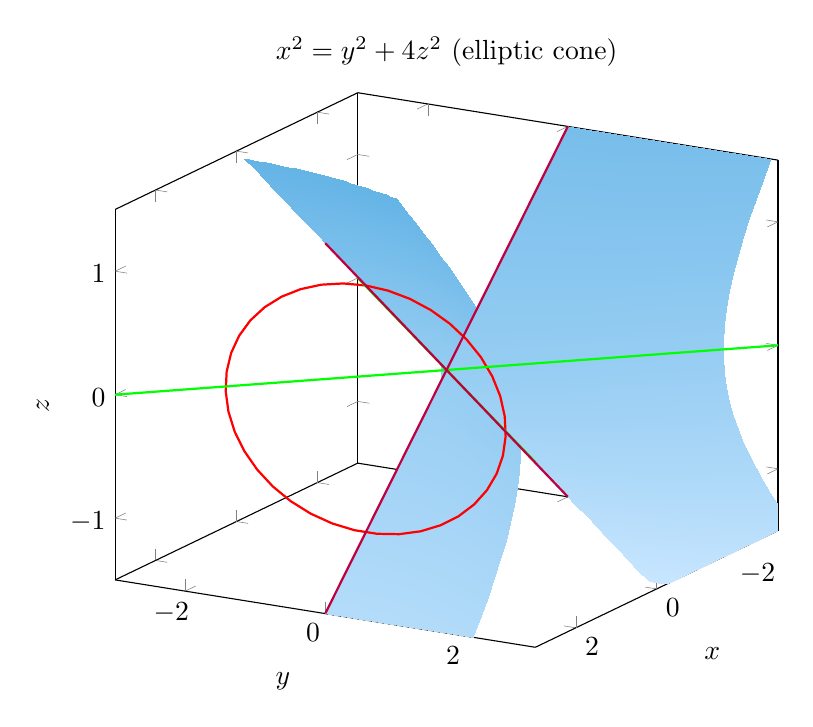
\begin{tikzpicture}
\begin{axis}[
    width=10cm,
    view={120}{20},
    xlabel={$x$}, ylabel={$y$}, zlabel={$z$},
    xmin=-3, xmax=3,
    ymin=-3, ymax=3,
    zmin=-1.5, zmax=1.5,
    samples=40,
    samples y=40,
    colormap={bluewhite}{rgb255=(200,230,255) rgb255=(100,180,230)},
    title={$x^2=y^2+4z^2$ (elliptic cone)}
]
\addplot3[surf, shader=interp, domain=0:2.5, domain y=-2.5:2.5] ({sqrt(x^2+4*y^2)},x,y);
\addplot3[surf, shader=interp, domain=0:2.5, domain y=-2.5:2.5] ({-sqrt(x^2+4*y^2)},x,y);
% Trace ellipse x=2 (in original coordinates: x=2, y^2+4z^2=4)
\addplot3[red, thick, samples y=0, domain=0:360] ({2},{2*sin(x)},{cos(x)});
% Trace lines in coordinate planes
\addplot3[green, thick, samples y=0, domain=-3:3] (x,x,0);
\addplot3[green, thick, samples y=0, domain=-3:3] (x,-x,0);
\addplot3[purple, thick, samples y=0, domain=-1.5:1.5] (2*x,0,x);
\addplot3[purple, thick, samples y=0, domain=-1.5:1.5] (-2*x,0,x);
\end{axis}
\end{tikzpicture}
\end{document}